%!TEX root = ../my_thesis.tex

\appendix

\chapter{Compléments au Chapitre 1}
\section{Détails 1}\label{append:decoding_nodes}

Les sorties du canal composite sont des informations souples données par le démodulateur.
Ce bruit additif est ajouté à la valeur des données en sortie du modulateur $\mathbold{x}$.
\begin{equation}
y_i = x_i + n_i
\end{equation}
Dans le modèle de chaine de communication considéré, la puissance du bruit du canal AWGN $N_0$ est supposée connue.
Cela permet au démodulateur de calculer la probabilité conditionnelle suivante.
\begin{equation}
	P_r( \tilde{y}_i|\tilde{x}_i) = \dfrac{1}{\sqrt{\pi N_0}}\exp^{-\tfrac{(\tilde{x}_i^2-\tilde{y}_i^2)}{N_0}}
\end{equation}
$p_i$ représente la probabilité de recevoir $\tilde{y}_i$ en présupposant la valeur de $\tilde{x}_i$ en sortie du modulateur ($\tilde{x}_i=-1$ ou $\tilde{x}_i=1$). Les \textit{log likelihood ratios} (LLRs), utilisés dans la chaîne de communication considérée dans cette thèse, sont exprimés en fonction de ces probabilités :
\begin{equation}
	L_i = \log\left(\dfrac{P_r(y_i | x_i = 0)}{P_r(y_i | x_i = 1)}
	\label{eq:lr}\right)
\end{equation}

Les codes correcteurs d'erreurs peuvent être définis par un ensemble de contraintes de parités. Une représentation graphique de ces contraintes est appelé \textit{graphe de Tanner} comme représenté en Figure~\ref{fig:noeuds}

\begin{figure}[t]
\centering
\includegraphics{tail/appendix_1_fig/noeuds}
\caption{Représentations des noeuds de décodage}
\label{fig:noeuds}
\end{figure}

Le noeud de parité est la représentation graphique de l'équation suivante : 
\begin{equation}
b_0 + b_1 + b_2 = 0
\end{equation}
Tandis que l'encodeur canal associe le vecteur d'entrée $\mathbold{b}$ de longueur $K$ à un mot de code $\mathbold{x}$ de longueur $N$, le décodeur combine les différents LLRs en sortie du canal composite dans le but de retrouver les bits d'origine.
Dans l'exemple de la Figure~\ref{fig:noeuds}, les estimations du canal pour les valeurs des bits $b_1$ et $b_2$, notés respectivement $L_1$ et $L_2$, peuvent être combinées afin de calculer une estimation extrinsèque du bit $b_0$, notée $L_0^e$.

Sa valeur est par définition :
\begin{equation}
L^e_0 = \dfrac{P(y_1,y_2 | b_0 = 0)}{P(y_1,y_2 | b_0 = 1)}
\label{eq:le0}
\end{equation}
Seules deux combinaisons possibles des bits $b_1$ et $b_2$ peuvent impliquer que $b_0$ soit égal à $0$ : ou bien $b_1=0$ et $b_2=0$, ou bien $b_1=1$ et $b_2=1$. Il est donc possible de calculer $P(b_0|y_1,y_2)$ : 
\begin{equation}
P(y_1,y_2 | b_0 = 0)  =  P(y_1 | b_1 = 0)P(y_2 | b_2 = 0) + P(y_1 | b_1 = 1)P(y_2 | b_2 = 1) \\
\end{equation}
Donc,  
\begin{equation}
P(y_1,y_2 | b_0 = 0)  =  L_1L_2 + 1 \\
\label{eq:le1}
\end{equation}


De la même manière,,
\begin{equation}
P(b_0 = 1 | y_1,y_2) =P(y_1 | b_1 = 0)P(y_2 | b_2 = 1) + P(y_1 | b_1 = 1)P(y_2 | b_2 = 0)
\end{equation}
Donc, 
\begin{equation}
P(b_0 = 1 | y_1,y_2) = L_1 + L_2
\label{eq:le2}
\end{equation}
On déduit donc de \ref{eq:le0}, \ref{eq:le1} et \ref{eq:le2} : 

\begin{equation}
L^e_0=\dfrac{1 + L_1L_2}{L_1+L_2}
\label{eq:parity}
\end{equation}

En effectuant la même démarche pour le N\oe{}ud d'égalité il est possible d'obtenir :
\begin{eqnarray*}
\begin{array}{r c l}
P(y_1,y_2|b_0=0) & = & P(y_1|b_1=0) P(y_2 | b_2 = 0) \\
P(y_1,y_2|b_0=1) & = & P(y_1|b_1=1) P(y_2 | b_2 = 1) 
\end{array}
\end{eqnarray*}
Il est possible d'en déduire l'extrinsèque :
\begin{equation}
L^e_0=L_1L_2
\label{eq:equality}
\end{equation}

L'algorithme de décodage SC peut être représenté sous la forme de \textit{factor graph} dans lequel les équations \ref{eq:parity} et \ref{eq:equality} sont appliquées, comme montré en Figure~\ref{fig:SCSchedule}


SC decoding sequentially use the equations  (\ref{eq:parity}) and (\ref{eq:equality}) to decode the polar code graph.
There are two levels of decoding: \textit{soft estimations} and \textit{hard decisions}. Soft decisions are mathematically represented by probabilities, likelihood ratios or log-likelihood ratios. In our examples and to use the former equations, likelihood ratios will represent soft estimation. The hard decisions are classically called partial sums and are mathematically represented by values in $\{0,1\}$ and are noted $S_{i,j}$ where $i$ represents the lane, and $j$ represents the stage (also called depth) of the partial sum in the factor graph. Same indexes notations are used for other objects in the graph. The introduction of these notations along with equality nodes will enrich the representation of the factor graph. The following figures represent the different decoding steps for a polar code of size $N=2$.

\begin{figure}[!ht]
  \centering
  \subfloat[][$F$ function]{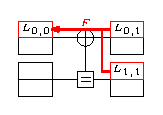
\includegraphics[width=.24\textwidth]{tail/appendix_1_fig/SC_graph2_b}}\quad\quad\quad\quad
  \subfloat[][$G$ function]{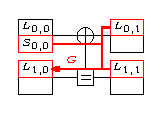
\includegraphics[width=.25\textwidth]{tail/appendix_1_fig/SC_graph2_d}}
  \caption{Fonctions $f$ et $g$ de l'algorithme SC}
  \label{fig:SCSchedule}
\end{figure}

Figure \ref{fig:SCSchedule} shows the sequence of the different operations of successive cancellation decoding algorithm:
\begin{itemize}
\item[(a)] The first step is the loading of the channel likelihood ratios into the decoding factor graph.
\item[(b)] The second step is the computation of the value of $L_{0,1}$. The function used is the computation of the extrinsic of a parity node as described in equation \ref{eq:parity}:
\begin{equation}
L_{0,0} = F(L_{0,1}, L_{1,1}) = \dfrac{1+L_{0,1}L_{1,1}}{L_{0,1}+L_{1,1}}
\end{equation}
\item[(c)] The third step is an hard decision to deduce $S_{0,0}$ from $L_{0,0}$:
 \[
    S_{0,0}=HD(L_{0,0})=
    	\begin{cases} 
    		0 & \text{if }L_{0,0}\geq0.5\\
    		1 & \text{if }L_{0,0}<0.5
    		\end{cases}
  \]
\item[(d)] The fourth step is the computation of the value of $L_{1,1}$. The inputs used are $S_{0,0}$, $L_{0,1}$ and $L_{1,1}$. We see that the equality node is used, so we will use the equality node equation (\ref{eq:equality}). The first member of the equation is $L_{1,1}$. The second member depends on the value of $S_{0,0}$.

\[
	L_{1,0} = 
	\begin{cases} 
	L_{1,1}L_{0,1} & \text{if }S_{0,0} = 0\\
	L_{1,1}\dfrac{1}{L_{0,1}} & \text{if }S_{0,0} = 1
	\end{cases}
\]

This can be simplified:
\begin{equation}
L_{1,0} = G(L_{1,1},L_{0,1},S_{0,0}) = L_{1,1}L_{0,1}^{1 - 2S_{0,0}}
\end{equation}
\item[(e)] Fifth step is an hard decision: 
\begin{equation*}
S_{1,0}=HD(L_{1,0})
\end{equation*}
\item[(f)] Final step is the propagation of the partial sums, which is equivalent to a polar encoder.
\begin{equation}
S_{0,1} = H_u(S_{0,0},S_{1,0}) =S_{0,0}\oplus S_{1,0}
\end{equation}	
\begin{equation}
S_{1,1} = H_l(S_{1,0}) = S_{1,0}\\
\end{equation}

	
\end{itemize}

\chapter{Compléments au Chapitre 2}\label{sec:annCCSDS}
\chapter{Compléments au Chapitre 3}\label{sec:ann3}
